\section{Phương pháp}
\subsection{Hồi Quy Tuyến Tính}
Hồi quy tuyến tính là một phương pháp dùng để dự đoán giá trị của một biến phụ thuộc dựa trên một hoặc nhiều biến độc lập.

Ta giả định rằng mối quan hệ giữa biến đầu vào và đầu ra là tuyến tính – tức là có thể biểu diễn bằng một đường thẳng.
\subsubsection*{Nguyên lý hoạt động:}
\begin{itemize}
    \item \textbf{Hồi quy tuyến tính đơn (1 biến đầu vào):}
    \[
        y = wx + b
    \]
    Trong đó:
    \begin{itemize}
        \item $y$: biến đầu ra (giá trị cần dự đoán)
        \item $x$: biến đầu vào
        \item $w$: hệ số góc (trọng số)
        \item $b$: hệ số chệch (bias / intercept)
    \end{itemize}
    
    \item \textbf{Hồi quy tuyến tính đa biến (n biến đầu vào):}
    \[
        y = w_1x_1 + w_2x_2 + \cdots + w_nx_n + b = \mathbf{w}^T \mathbf{x} + b
    \]
    Với:
    \[
        \mathbf{x} = [x_1, x_2, \ldots, x_n]^T,\quad \mathbf{w} = [w_1, w_2, \ldots, w_n]^T
    \]
\end{itemize}
Để đo độ chính xác của mô hình, ta thường dùng hàm MSE (Mean Squared Error):
\[
    \text{MSE} = \frac{1}{m} \sum_{i=1}^{m} \left( y^{(i)} - \hat{y}^{(i)} \right)^2
\]
Trong đó:
\begin{itemize}
    \item $m$: số lượng mẫu
    \item $y^{(i)}$: giá trị thực tế của mẫu thứ $i$
    \item $\hat{y}^{(i)}$: giá trị dự đoán của mô hình với mẫu thứ $i$
\end{itemize}

Mô hình hồi quy tuyến tính là một phương pháp phù hợp cho bài toán dự báo giá nhà vì nó giúp mô tả mối quan hệ giữa các yếu tố như diện tích, số phòng,... và giá trị của căn nhà bằng một hàm tuyến tính đơn giản. Trong thực tế, giá nhà thường biến đổi theo xu hướng tuyến tính đối với những đặc trưng này, nên mô hình không chỉ cho kết quả dự đoán khá chính xác mà còn dễ dàng giải thích được tác động của từng yếu tố đến giá. Tính đơn giản, dễ huấn luyện và khả năng diễn giải rõ ràng khiến hồi quy tuyến tính trở thành lựa chọn hiệu quả cho các hệ thống dự báo giá trong lĩnh vực bất động sản.

\subsection{Random Forest}
Random Forest là phương pháp kết hợp các dự đoán của nhiều cây quyết định để tạo ra kết quả chính xác và ổn định hơn. Nó có thể được sử dụng cho cả phân loại và hồi quy.

Trong hồi quy (Random Forest Regression), mô hình được sử dụng để dự đoán giá trị liên tục. Thay vì bỏ phiếu, các cây quyết định đầu ra một giá trị số, và kết quả cuối cùng là trung bình của tất cả các dự đoán từ các cây trong rừng.
\subsubsection*{Nguyên lý hoạt động:}

Random Forest Regression hoạt động bằng cách kết hợp nhiều cây hồi quy \( f_1(x), f_2(x), \ldots, f_T(x) \), mỗi cây được huấn luyện trên một tập dữ liệu ngẫu nhiên khác nhau. Tập dữ liệu huấn luyện cho mỗi cây \( f_t \) được tạo thông qua phương pháp \textbf{Bootstrap Sampling} từ tập dữ liệu gốc \( D \):

\[
D_t \sim \text{Bootstrap}(D), \quad t = 1, 2, \ldots, T
\]

Ngoài ra, tại mỗi nút trong cây, chỉ một tập con ngẫu nhiên các đặc trưng \( \mathcal{F}_t \subseteq \mathcal{F} \) được lựa chọn để tìm điểm chia, nhằm tăng tính đa dạng giữa các cây.

Quá trình xây dựng cây diễn ra bằng cách đệ quy phân chia tập dữ liệu dựa trên giá trị của một đặc trưng sao cho giảm thiểu sai số dự đoán. Hàm mất mát phổ biến trong hồi quy là tổng bình phương sai số (Sum of Squared Errors - SSE), được tối ưu tại mỗi nút:

\[
\text{SSE} = \sum_{i \in S} \left( y^{(i)} - \bar{y}_S \right)^2
\]

với \( S \) là tập mẫu tại nút hiện tại, và \( \bar{y}_S \) là giá trị trung bình của biến mục tiêu tại tập \( S \):

\[
\bar{y}_S = \frac{1}{|S|} \sum_{i \in S} y^{(i)}
\]

Tiêu chí dừng cho mỗi cây có thể bao gồm: độ sâu tối đa, số lượng mẫu tối thiểu tại nút, hoặc mức độ giảm sai số không đáng kể.

Sau khi huấn luyện, mỗi cây hồi quy \( f_t(x) \) đầu ra một giá trị số thực. Dự đoán cuối cùng của Random Forest Regression là trung bình các dự đoán từ tất cả các cây:

\[
\hat{y} = \frac{1}{T} \sum_{t=1}^{T} f_t(x)
\]

Trong đó:

\begin{itemize}
    \item \( T \): số lượng cây trong rừng
    \item \( f_t(x) \): dự đoán của cây thứ \( t \) với đầu vào \( x \)
    \item \( \hat{y} \): giá trị dự đoán cuối cùng của mô hình
\end{itemize}

\begin{figure}[H]
    \centering
    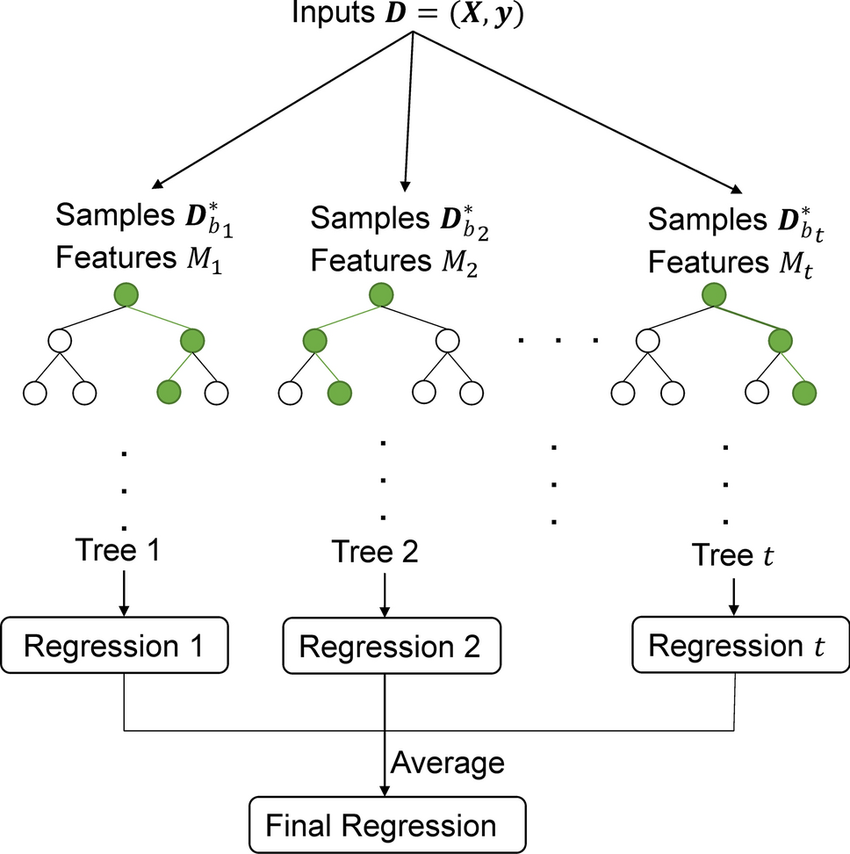
\includegraphics[width=0.8\textwidth]{chapters/PP/assets/Concept-of-a-random-forest-regression-model-after-14.png}
    \caption{Random Forest}
    \label{fig:enter-label}
\end{figure}

Random Forest là sự lựa chọn thích hợp cho bài toán dự đoán giá nhà vì khả năng mô phỏng các quan hệ phi tuyến phức tạp giữa các yếu tố như diện tích, vị trí và số phòng, điều mà hồi quy tuyến tính không thể làm tốt. Mô hình này không yêu cầu giả định về mối quan hệ giữa các biến và có thể xử lý tốt với dữ liệu thiếu sót hoặc không đồng nhất. Random Forest cũng tự động chọn ra các đặc trưng quan trọng, giúp cải thiện độ chính xác của dự đoán. Bên cạnh đó, nhờ việc kết hợp nhiều cây quyết định, mô hình này giảm thiểu được hiện tượng overfitting, mang lại kết quả ổn định và chính xác hơn so với các mô hình tuyến tính trong việc dự đoán giá nhà.

\subsection{XGBoost}
XGBoost (Extreme Gradient Boosting) là một thuật toán học máy mạnh mẽ thuộc nhóm ensemble learning, cụ thể là phương pháp boosting. Nó được thiết kế để tối ưu hiệu năng và tốc độ khi huấn luyện mô hình cây quyết định.
\subsubsection*{Nguyên lý hoạt động:}
XGBoost xây dựng mô hình bằng cách kết hợp nhiều cây quyết định theo từng vòng lặp. Mỗi cây mới được huấn luyện nhằm sửa lỗi của cây trước đó, giúp mô hình học tốt hơn theo thời gian.

\subsubsection*{1. Hàm mục tiêu}

Ở vòng boosting thứ \( t \), mô hình XGBoost tối ưu hàm mục tiêu sau:
\[
\mathcal{L}^{(t)} = \sum_{i=1}^{n} l(y_i, \hat{y}_i^{(t-1)} + f_t(x_i)) + \Omega(f_t)
\]

Trong đó:
\begin{itemize}
    \item \( l \): hàm mất mát (thường dùng MSE: \( l(y, \hat{y}) = (y - \hat{y})^2 \))
    \item \(\hat{y_i}^{(t-1)}\): dự đoán của mô hình tại bước t - 1
    \item \(f_t\): cây quyết định mới tại bước t
    \item \( \Omega(f_t) \): thành phần regularization giúp chống overfitting
\end{itemize}

\[\Omega(f)f_t  = \gamma T + \frac{1}{2} \lambda \sum_{j=1}^{T} w_j^2 \]

Trong đó:
\begin{itemize}
    \item \(T\): số lá của cây
    \item \(w_j\): trọng số lá thứ \(j\)
    \item \(\gamma, \lambda\): hệ số điều chỉnh độ phức tạp mô hình
\end{itemize}
\subsubsection*{2. Xấp xỉ Taylor bậc hai}

XGBoost sử dụng xấp xỉ Taylor bậc hai để làm trơn hàm mất mát:

\[
\mathcal{L}^{(t)} \approx \sum_{i=1}^{n} \left[ g_i f_t(x_i) + \frac{1}{2} h_i f_t^2(x_i) \right] + \Omega(f_t)
\]

Trong đó:
- \( g_i = \frac{\partial l(y_i, \hat{y}_i^{(t-1)})}{\partial \hat{y}_i^{(t-1)}} \) (đạo hàm bậc 1)
- \( h_i = \frac{\partial^2 l(y_i, \hat{y}_i^{(t-1)})}{\partial (\hat{y}_i^{(t-1)})^2} \) (đạo hàm bậc 2)

\subsubsection*{3. Tính giá trị tối ưu tại mỗi lá}

Với mỗi lá \( j \), tập mẫu thuộc lá là \( I_j \). Tổng gradient và hessian tại lá:

\[
G_j = \sum_{i \in I_j} g_i, \quad H_j = \sum_{i \in I_j} h_i
\]

Giá trị đầu ra tối ưu tại lá:

\[
w_j^* = -\frac{G_j}{H_j + \lambda}
\]

Giá trị hàm mục tiêu tại điểm cực tiểu:

\[
\mathcal{L}^{(t)} = -\frac{1}{2} \sum_{j=1}^{T} \frac{G_j^2}{H_j + \lambda} + \gamma T
\]

\subsubsection*{Quá trình huấn luyện:}
Quá trình huấn luyện XGBoost bao gồm các bước chính sau:

\begin{itemize}
    \item[1. ] \textbf{Khởi tạo mô hình:} Dự đoán ban đầu là giá trị trung bình (cho hồi quy) hoặc xác suất (cho phân loại).
    \item[2.] \textbf{Tính toán gradient và hessian:} Các gradient (\( g_i \)) và hessian (\( h_i \)) được tính cho mỗi mẫu dựa trên hàm mất mát.
    \item[3.] \textbf{Xây dựng cây quyết định:} Mỗi cây mới được xây dựng để tối ưu hóa hàm mất mát với việc sử dụng gradient và hessian.
    \item[4.] \textbf{Cập nhật dự đoán:} Dự đoán của mô hình được cập nhật bằng cách cộng thêm giá trị từ cây mới.
    \item[5.] \textbf{Regularization:} Thành phần regularization giúp kiểm soát độ phức tạp của mô hình và ngăn ngừa overfitting.
    \item[6.] \textbf{Lặp lại quá trình:} Các bước trên được lặp lại cho đến khi đạt số vòng lặp tối đa hoặc không còn cải thiện đáng kể.
\end{itemize}

XGBoost là một lựa chọn mạnh mẽ cho bài toán hồi quy dự đoán giá nhà nhờ vào khả năng xử lý các mối quan hệ phi tuyến tính phức tạp trong dữ liệu. Mô hình này sử dụng kỹ thuật boosting, giúp tăng cường độ chính xác qua từng vòng lặp bằng cách học từ các sai sót của các cây quyết định trước đó. Điều này giúp XGBoost cải thiện hiệu suất so với mô hình hồi quy tuyến tính, vốn chỉ phù hợp với mối quan hệ tuyến tính giữa các đặc trưng và giá trị dự đoán.

Khác biệt với Random Forest, XGBoost không chỉ tạo ra nhiều cây quyết định độc lập mà còn tập trung vào việc tối ưu hóa mỗi cây dựa trên gradient của hàm mất mát, giúp giảm sai số một cách hiệu quả. Mặc dù Random Forest có thể xử lý các mối quan hệ phi tuyến tính, nhưng XGBoost thường cho kết quả tốt hơn nhờ vào khả năng tối ưu hóa liên tục và điều chỉnh chính xác hơn qua mỗi vòng huấn luyện.

\subsection{GridSearchCV} 
GridSearchCV là một phương pháp được sử dụng để tìm kiếm và tối ưu các siêu tham số (hyperparameters) của một mô hình học máy, nhằm cải thiện độ chính xác và hiệu suất của mô hình. Nó thực hiện thử tất cả các tổ hợp các giá trị siêu tham số có thể có từ một "lưới" các giá trị đã được chỉ định trước.

\subsubsection*{Nguyên lý hoạt động:}
GridSearchCV tìm kiếm trong không gian siêu tham số bằng cách thử nghiệm với mọi giá trị của các tham số đã cho, sử dụng phương pháp k-fold cross-validation để đánh giá hiệu suất của mỗi kết hợp tham số. Mục tiêu là tìm ra bộ tham số có thể tối ưu hóa độ chính xác của mô hình.

Quá trình này có thể được mô tả như sau:
\[
\text{Best Parameters} = \arg \max_{\theta} \left( \frac{1}{k} \sum_{i=1}^{k} \text{score}(X_{train}^{(i)}, y_{train}^{(i)}, \theta) \right)
\]
Trong đó:
\begin{itemize}
    \item \( \theta \) là bộ tham số của mô hình.
    \item \( X_{train}^{(i)} \) và \( y_{train}^{(i)} \) là dữ liệu huấn luyện tại lần gập thứ \(i\) trong quá trình k-fold cross-validation.
    \item \(\text{score}(X, y, \theta)\) là độ chính xác của mô hình với tham số \(\theta\) trên bộ dữ liệu \(X\) và \(y\).
\end{itemize}
\subsubsection*{Tối ưu siêu tham số với GridSearchCV}
Trong bài toán này, nhóm sẽ kết hợp giữa phương pháp bagging và boosting cây quyết định, cụ thể là các mô hình Random Forest và XGBoost, với kỹ thuật GridSearchCV để tối ưu hóa các tham số của mô hình. Phương pháp bagging (Bootstrap Aggregating) được áp dụng với Random Forest, trong khi đó boosting được sử dụng với XGBoost, nhằm tăng cường hiệu quả dự đoán và giảm thiểu lỗi.

Cả hai mô hình Random Forest và XGBoost đều có các siêu tham số quan trọng có thể điều chỉnh để tối ưu hóa hiệu suất. Với GridSearchCV, nhóm sẽ tìm kiếm và chọn lựa các giá trị siêu tham số tối ưu thông qua việc thử nghiệm tất cả các kết hợp có thể của các tham số trong không gian tìm kiếm. Quá trình này giúp mô hình đạt được hiệu quả dự đoán tốt nhất cho bài toán cụ thể.

GridSearchCV sẽ giúp tìm ra các tham số tối ưu của mô hình thông qua việc đánh giá hiệu suất mô hình trên một tập kiểm tra (cross-validation) với các tham số khác nhau, từ đó chọn ra bộ tham số tối ưu giúp mô hình hoạt động hiệu quả nhất. Các tham số sẽ bao gồm:
\begin{itemize}
    \item \textbf{Random Forest:} số lượng cây (\textit{n\_estimators}), độ sâu tối đa của cây (\textit{max\_depth}), số lượng mẫu tối thiểu để chia tách (\textit{min\_samples\_split}).
    \item \textbf{XGBoost:} số lượng cây (\textit{n\_estimators}), tốc độ học (\textit{learning\_rate}), độ sâu của cây (\textit{max\_depth}), tỷ lệ mẫu (\textit{subsample}).
\end{itemize}

Việc kết hợp giữa bagging, boosting và GridSearchCV giúp mô hình cải thiện khả năng dự đoán trong các bài toán phức tạp như dự báo giá nhà, từ đó giúp mô hình có khả năng học được các mối quan hệ phi tuyến tính và giảm thiểu overfitting.

